\documentclass[a4paper]{article}
\usepackage{mathtools}
\usepackage{verbatim}
\usepackage{graphicx}
\usepackage{tabularx}
\usepackage{pgfplots}
\usepackage{adjustbox}
\usepackage{booktabs}
\makeatletter
\let\latex@xfloat=\@xfloat
\def\@xfloat #1[#2]{%
    \latex@xfloat #1[#2]%
    \def\baselinestretch{1}
    \@normalsize\normalsize
    \normalsize
}
\makeatother
\usepackage{amsmath}
\usepackage{mathtools}
\usepackage{epigraph}
\usepackage{cancel}
\usepackage{xcolor}
\newcommand\Ccancel[2][black]{\renewcommand\CancelColor{\color{#1}}\cancel{#2}}
\usepackage{graphicx}
\usepackage[utf8]{inputenc}
\usepackage{pgfplots}
\usepackage{tabularx}
\DeclareUnicodeCharacter{2212}{−}
\usepgfplotslibrary{groupplots,dateplot}
\usetikzlibrary{patterns,shapes.arrows}
\pgfplotsset{compat=newest}
\begin{document}
\begin{titlepage}

    \title{
    Update Report}


    \author{ Jeffrey Severino \\
        University of Toledo \\
        Toledo, OH  43606 \\
    email: jseveri@rockets.utoledo.edu}


    \maketitle

\end{titlepage}
\section{Current Research Direction}
The goal is to clarify what occurs when ducts are lined 
with sound absorbing material.  Speciificaally, the description of acoustic liner
in terms of the Linearized Euler Equations is investigated.
\section{Research Performed}
The acoustic absorbing material is called locally reacting and is often 
describes with ``wall impedance'' and will be denoted as $Z(\omega)$

The boundary condition is given as

\[i \omega p = -Z \frac{\partial p'}{\partial r} \text{at} r = 1 \]

A typical test case example is for the inlet of an aircraft turbojet engine. 
The general solution has a form similar to the hard wall case, except the 
eigenvalues $k_r$ are now defined by

\[\frac{J_m(k_r) }{k_r J'_m (k_{r,mn})} = \frac{ i Z}{\omega}\]

Which is related to $k_{x}$ by 

\[k_{x}^{\pm} =  \pm \sqrt{ k^2 - k_{r,mn}} = \pm \omega \zeta(k_{r,mn}/\omega)\]

While these ``soft wall'' modes are no longer orthoganal, the modes could be normalized in such a way
that preserves the normalization relation,

\[ \int_0^1 U_{mn} (r) \text{conj}(U_{mn}(r)) r d\Theta dr = 1 \]

The normalization constan 
\[N_{mn} = \frac{|Z|}{|J_m(k_{r,mn}|} \sqrt{\frac{Im(k_{r,mn}^2}{\omega Re(Z)}}\]


\section{Issues and Concerns}
The new function $\zeta$ is described in Rienstra's work in his appendix in a clever way\dots


He defines $\zeta$ as a function of an arbitrary number $z$.

\[\zeta(z) = \sqrt{1 - z^2}\]

where $Im(\zeta) \leq 0$, and $\zeta(0) = 1$

His description is,

`` 
The sign choice is made such that always $Im(\zeta) \leq 0$. This implies that the branch cuts 
are located right along the curves where $Im(\zeta) = 0$. i.e. along the imaginary 
axis, and the real interval $|z| \leq 1$.
For definiteness the branch cuts are included in the dommain of the 
definition as the limits from the $Re \zeta > 0$ side. 
If we take care along the branch cuts, where sign($Im \zeta$) is not defined,
a simple (theres a footnote  here) way to determine $\zeta$ is 

\[ \zeta(z) = - sign (Im \sqrt{1 - z^2}) \sqrt{1 - z^2} \]

"
There is a nice figure shown along with this description 
\begin{figure}[!]
    \centering
    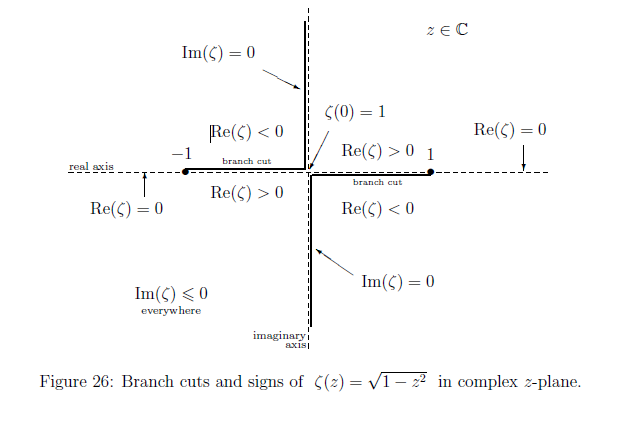
\includegraphics{Capture.PNG}
    \caption{Fiigure in appendix A.2 An Important Complex Square Root in 
    Fundamentals of Duct Acoustics by Rienstra}
\end{figure}
\section{Planned Research}

I am slightly confused on how to use this information.. but my current understanding 
of this is that the value of $Z$ changes which zero zrossings $k_r$ are used.


\end{document}


